\documentclass[11pt, twocolumn]{article}
\usepackage[margin=1in]{geometry}
\usepackage{graphicx}
\usepackage{amsmath}
\usepackage{hyperref}

%opening
\title{Modeling Superspreading using Branching Processes and Networks}
\author{William Magrogan}

\begin{document}

\maketitle

\begin{abstract}
Stochastic branching models are a useful tool for understanding the behavior of superspreading and superspreaders in the context of epidemological outbreaks. In this paper, we explore the behavior of extremely overdispersed, heavy-tailed distributions on the dynamics of outbreaks and compare them to standard models of superspreading and standard Poissonian distributions. In particular, we focus in on the basic reproductive number, $R_0$, the probabilities of major and minor outbreaks, and the size distribution of minor outbreaks.
\end{abstract}

\section*{Introduction}
Superspreading events (SEV) and superspreaders (SS) have been identified as important processes to understanding the spreading of some pathogens such as SARS-CoV-2. SEVs are understood as instances of time with an anomalously high rate of secondary infections by a primary infector. Similarly, an SS is understood as an individual associated with a high secondary infection rate. When they occur, SEVs are rarer, but the degree of secondary infections can often lead to outbreaks simply by the number of new transmission vectors introduced. For certain pathogens, SEVs and SSs are critical to understanding their spread and outbreak behavior. While there are many mathematical tools available to model and analyze this behavior, stochastic branching processes are particularly useful.\\ \\
Stochastic models have the advantages of being flexible, having a robust way to integrate uncertainty about model processes, and often times makes comparison with real-world data simpler. In previous works \cite{??}, branching processes have been used to model SEVs in SARS-CoV-2 data and determine that $R_0$ distributions following a negative binomial distribution fit the data well. Negative binomial distributions have a particularly high variance, which agrees with observations of human network structure. \\ \\
Some models of network formation \cite{barabasi, yule, polya} suggest contact structures (degree distributions) may have even greater variance than, say, a negative binomial distribution. Here, we are interested in comparing superspreading in these contexts to those of standard overdispersion.

\section*{Background}
Stochastic branching processes have been used to study concrete biological processes to extinction of surnames \cite{last names guy}. This can be thought of as a Galton-Wattson process where $Z_j$ denotes the number of elements in generation $j$ and $X_{j, k}$ is the number of successors of member $k$ from generation $j$, then 
\begin{equation}
	Z_{j+1} = \sum_{k=0}^{Z_j}X_{j,k}. \label{eqn:GW}
\end{equation}
In the case of epidemics, $Z_j$ is the number of infected elements in generation $j$, and $X_{j, k}$ is a random variable (RV) describing how many people they infect, or the secondary number of infections. The important dynamics lay in how $X_{j,k}$ is realized.\\ \\
The three elements of this model that determine $X_{j,k}$ are number of secondary contacts, probability of infection, and vaccination. For the extremely overdispersed model, a Yule RV will be used. This is motivated from the Albert-Barabasi model of network growth accounting for preferential attachment processes. Yule RVs have

\begin{equation}
	f_{Yule(\rho)}(k)=
	\begin{cases}
		\rho B(k, \rho+1)& k \in \{1, 2, \ldots\}\\
		0&\text{otherwise}.
	\end{cases}
\end{equation}
Here, we will use $\rho=2$, which gives asymptotic decay as $k^{-3}$. Note that the variance is undefined since
\begin{equation}
	\sum_{k\geq 1}\rho k B(k, 3)
\end{equation}
diverges. The mean is defined and $\langle k \rangle =2$. \\ \\
Next, the infectiousness, $p$, or probability of a pathogen being transmitted upon a contact, will be Beta distributed. A Beta distribution is supported on $[0,1]$ and has
\begin{equation}
	f_{Beta(\alpha, \beta)}(p)=\begin{cases}
	\frac{p^{\alpha-1}(1-p^{\beta-1})}{B(\alpha, \beta)}&p\in[0,1]\\
	0&\text{otherwise}.
	\end{cases}
\end{equation}
This is chosen to represent the variability in the infectiousness of a particular strain of the transmissible pathogen between hosts and the variability in host behavior that leads to transmission. Finally, vaccination should be accounted for. \\ \\
The two common models of vaccination are 'leaky' and 'all-or-nothing'. These are accounted for in the usual way of vaccine efficacy conferring probabilistic immunity or fractional immunity respectively. With these in place, we can build the model.

\subsection*{$R_0$ Calculation}
In the context of Epidemiology, $X_{j,k} = X$ can be interpreted as the number of secondary infections, we have dropped the indices since all primary infectors are pulled from the same distribution. Then $R_0$ is interpreted as the expected number of secondary infections. We may define a tool called an ordinary generating function (OGF), that is
\begin{equation*}
	G(q)\equiv\sum_{j\geq 0}q^j * Pr(X=j).
	\label{eqn:ogf}
\end{equation*}
This has some useful properties, in particular
\begin{enumerate}
	\item $G(0)=Pr(X=0)$
	\item $G(1)=1$
	\item $G'(1)=R_0$
\end{enumerate}
where the last property comes from a term-by-term differentiation of Eq. \ref{eqn:ogf}. In other words, $G(q)$ encodes all of the relevant information about the secondary infection distribution. It is also useful in calculation of minor outbreak probabilities.
\subsection*{Minor Outbreak Probability}
A minor outbreak in this context is an outbreak that such that $\lim_{n\rightarrow 0}Z_n=0$, or in other words, the outbreak eventually dies. Knowing if an outbreak eventually dies out is of practical importance, but also gives an estimate of probability of a major outbreak as $1-q$ where $q$ is the minor outbreak probability. Mathematically, since each instance of secondary infections is independent in this model, $q$ is calculated as
\begin{align}
	q = \sum_{j\geq 0}q^jPr(X=j) = G(q).
\end{align}
Then $q$ is just a fixed point of the OGF, specifically, the root of $G(q)-q=0$, which is how it will be calculated numerically. Note that $q=1$ is always a root, so we need to find the root $q^*\in (0, 1)$.
\section*{Models and Methods}
From here on, the model will be called the Extreme Overdispersion Model (EOD). In this branching model, $X_{j, k}$ from Eq. \ref{eqn:GW} as follows:
\begin{enumerate}
	\item Determine the number of contacts as $k = Yule(3)$.
	\item Determine the number of vaccinated contacts from the vaccination rate $v$ as $q = Binom(k, v)$.
	\item The infectiousness of the primary contact, $p$, is given by $p = Beta(\alpha, \beta)$.
	\item The number of susceptible infected is the $i_1 = Binom(k-q, p)$.
	\item If the vaccine is 'all-or-nothing' with efficacy $VE$, then $i_2 = Binom(q, VE)$.
	\item If the vaccine is 'leaky', then $i_2 = Binom(q, p(1-VE))$.
	\item Secondary infections are determined by $s=i_1+i_2$.
\end{enumerate}
The probability mass function (PMF) for $X_{j, k}$ without vaccination can be written down in terms of special functions as,

\begin{equation*}
	Pr(x_{j, k}=n)=\sum_{k\geq n}\rho B(k, \rho+1)\frac{B(\alpha+n, \beta+k)}{B(\alpha, \beta)}
\end{equation*}

 but will not be of much analytical help, similarly for the PMF for 'leaky' or 'all-or-nothing'. All of the behavior of the EOD model is determined by Monte-Carlo simulation (MCS) in Python and Numpy / Scipy packages. It is important to note that since the $Yule(3)$ RV is asymptotically a power law distribution, MCSs involving moments higher than $1$ will not converge. \\ \\
$R_0$ for the EOD model is calculated as the expected number of secondary infections. Since it is a first moment of the secondary infection distribution, there are no issues with their calculation. \\ \\
For a fair comparison between EOD and NB models, we need to find a common region of $R_0$, which are necessarily determined by MCS. This requires a sweep of $\alpha, \beta$ in the Beta RV and find a region of similar $R_0$. The Yule and NV RVs both have mean set to $2$, and this leaves the variance of the NB RV to vary and compare to the unbounded variance of the Yule RV.\\ \\
\subsection*{Calculating Minor Outbreak Probabilities}
To compute minor outbreak probabilities, realizations of secondary contacts are collected from multiple simulations. These are then converted into frequencies and used as a proxy to estimate the underlying secondary infection distribution. Using the frequencies as coefficients for the OGF in Eq. \ref{eqn:ogf}, $G(q)-q=0$ is solved using standard $1$D root finding methods, the BrentQ method in this study. Care needs to be taken during the root find since if $R_0<1$, the solver converges to the root at $1$, that is, only minor outbreaks can occur.
\section*{Results}
\subsection{Sensitivity of $R_0$ To Infection Parameters}
\begin{figure}
	\centering
	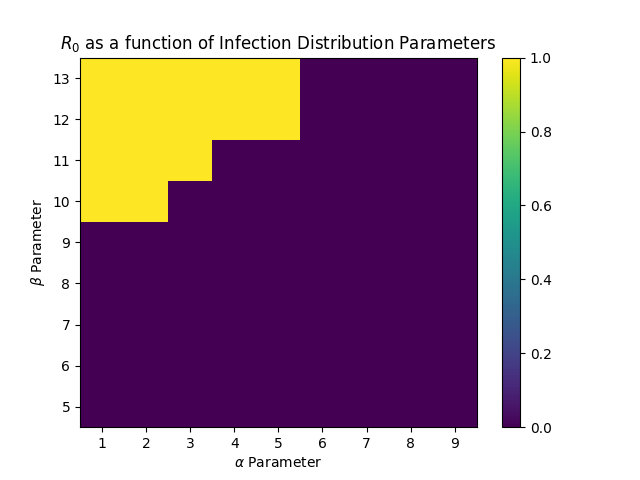
\includegraphics[scale=0.5]{YuleNoVaccSweep.png}
	\caption{$R_0$ as a function of $\alpha, beta$. Contact distribution is Yule with $\rho=2$}.
		\label{fig:yulesweep}
\end{figure}
\begin{figure}
	\centering
	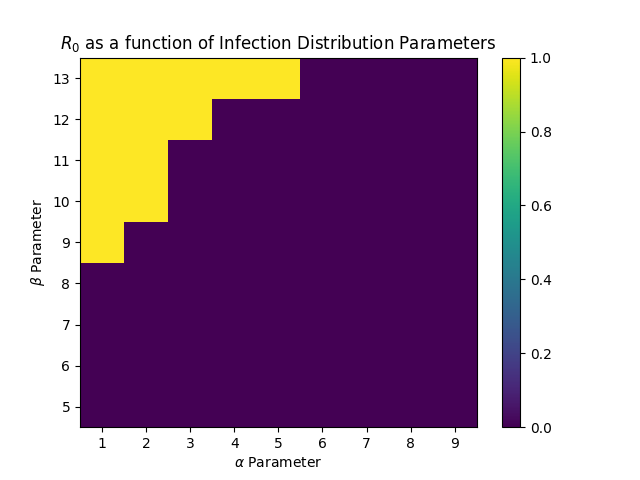
\includegraphics[scale=0.5]{NBNoVaccSweep.png}
	\caption{$R_0$ as a function of $\alpha, beta$. Contact distribution is NB with$\sigma^2=100$}.
	\label{fig:nbsweep}
\end{figure}
From Figs. \ref{fig:nbsweep}, \ref{fig:yulesweep}, we identify $(\alpha, \beta)=(12, 3)$ as a region for which both the Yule and NB contract distributions have close $R_0$ that is greater than $1$, which permits the possibility of major outbreaks that take hold in the population. This tells us that, according to Fig. \ref{fig:betadist}, a relatively large infectiousness is needed for major outbreaks to happen when the mean number of contacts is just $2$. In this case, $\langle p\rangle=0.8$.\\ \\

\begin{figure}
	\centering
	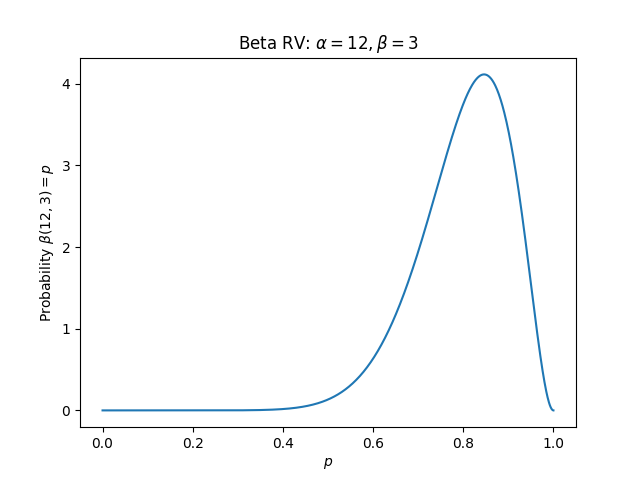
\includegraphics[scale=0.5]{betadist.png}
	\caption{Beta distribution PDF with parameters $\alpha=12, \beta=3$}. This indicates that relatively high and localized infectiousness parameters are needed to achieve $R_0\geq 1$.
	\label{fig:betadist}
\end{figure}

Recall that calculations of $R_0$ are taken from MCS, so there is necessarily noise around each calculation. We set $\beta=3$ fixed and increase $\alpha$ in the $R_0>1$ region. Note that the contact distributions both remain at $\langle k \rangle = 2$ average secondary contacts. Fig. \ref{fig:r0prog} demonstrates that for both NB and Yule distributed contact structures, $R_0$ increases at roughly the same rate, accounting for the noise. Interestingly, the variance in the EOD model and the overdispersed model seems to have little effect on the asymptotic behavior of $R_0$ as the pathogen becomes perfectly infectious.

\begin{figure}
	\centering
	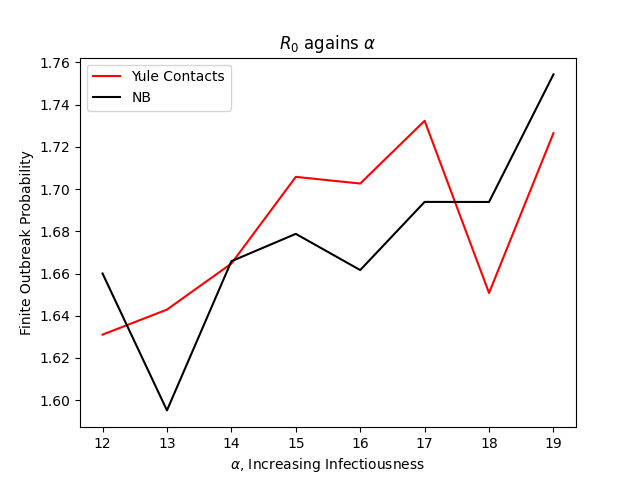
\includegraphics[scale=0.5]{nb_yule_r0.png}
	\caption{$R_0$ increases at roughly the same rate as for NB and Yule contact distributions $\alpha$ progresses and average infectiousness increases towards $1$.}
	\label{fig:r0prog}
\end{figure}

\subsection*{Sensitivity of $q$ To Infection Parameters}
We find an interesting result for the minor outbreak probability, $q$. Fig. \ref{fig:minoroutbreaks} demonstrates that the EOD model, for very similar values of $R_0$ and $\langle k \rangle$ have drastically different rates of minor outbreaks. This is interesting since it presents a clear delineation effects due to pathogenic infectiousness and the social structure of the host. This should not be too surprising, since the NB RV has exponential decay for large $k$, and Yule has algebraic decay, so naturally, very large secondary contacts occur more often for a Yule RV. Note that for the Yule contact structure, the estimate of $q$ slightly overestimates the realized minor outbreak rate. This is in part because the secondary infection distribution is naively estimated using frequencies, and in part due to the fact that some minor outbreaks are mis-identified as major outbreaks since only $5$ generations are realized for computational efficiency. For the NB, the estimate is very good to the simulation, and almost all outbreaks are minor ones in the simulation.

\begin{figure}
	\centering
	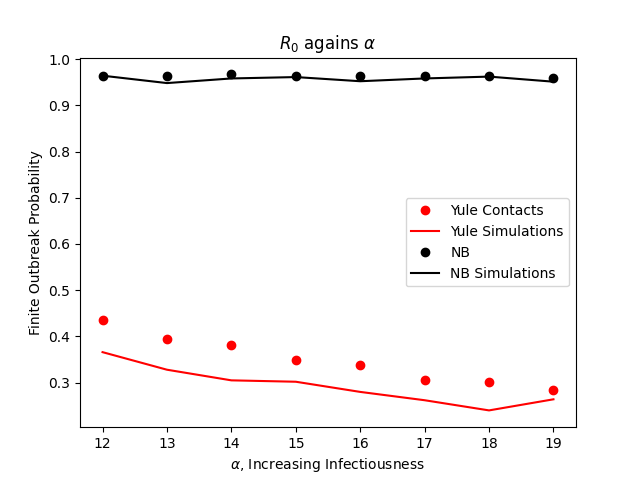
\includegraphics[scale=0.5]{nb_yule_finite_outbreaks.png}
	\caption{The Yule contact distribution has significantly lower minor outbreak probabilities than the NB contact structure.}
	\label{fig:minoroutbreaks}
\end{figure}

\subsection*{Sensitivity of $q$ To Vaccination Parameters}
Now, we want to consider the effect of 'leaky' versus 'all-or-nothing' vaccination models. Because $\rho=2$ is needed for the EOD model to exhibit unbounded variance, to compare EOD and NB models in the same $R_0$ regime, the NB model has minor outbreak probability $1$. So, In this section, the vaccination models will be compared only in the EOD model. The parameters ran in the model have $\alpha=20, \beta=3$ so that the EOD model has a small chance of minor outbreaks. The vaccine efficacy is set to $0.8$, and the vaccinated fraction of the population is varied from $0$ to $0.5$ The results for both models, simulations and estimates, are shown in Fig. \ref{fig:vacccomp}.

\begin{figure}
	\centering
	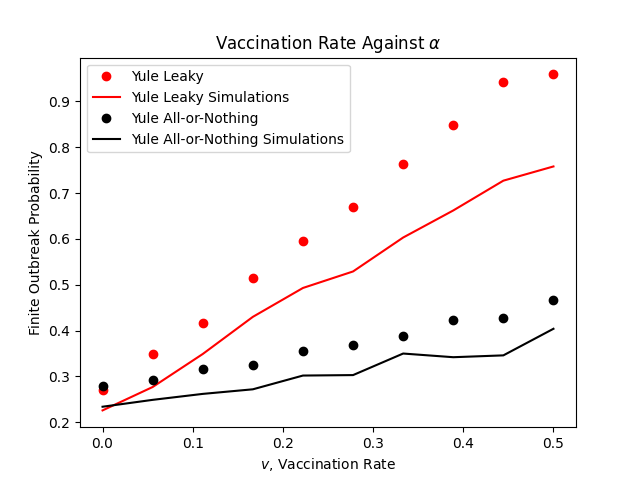
\includegraphics[scale=0.5]{YuleVaccComparison.png}
	\caption{The Yule contact distribution has significantly lower minor outbreak probabilities than the NB contact structure.}
	\label{fig:vacccomp}
\end{figure}

Note, again, the estimates are consistently high for the EOD model for reasons mentioned earlier. For both vaccination models, when $v=0$, they are equivalent, so they are comparable for small vaccination fraction. They both begin to differ significantly. Recall that 'leaky' vaccines provide partial immunity to all people vaccinated. Fig. \ref{fig:vacccomp} seems to indicate that 'leaky' vaccines are more effective in mitigating large outbreaks under the EOD model than 'all-or-nothing' vaccines in this regime. Its rather significant difference to the point where, under a 'leaky' vaccine, a vaccination rate of $~0.45$ completely eliminates major outbreak events, but the 'all-or-nothing' vaccine still has more than a $0.5$ chance of a major outbreak at the same level.

\section*{Discussion}
\section*{References}
\section*{Appendix}
Code used for simulations and figures available on github  \href{https://github.com/WilliamMagrogan/InfectiousDiseaseModeling}{here}, or you can also email the author at william.magrogan@colorado.edu.
\end{document}
